\documentclass[11pt,letterpaper]{article}
\usepackage{fullpage}
\usepackage[top=2cm, bottom=4.5cm, left=2.5cm, right=2.5cm]{geometry}
\usepackage{amsmath,amsthm,amsfonts,amssymb,amscd}
\usepackage{lastpage}
\usepackage{enumerate}
\usepackage{enumitem}
\usepackage{fancyhdr}
\usepackage{graphicx}
\usepackage{listings}
\usepackage{hyperref}
\usepackage{booktabs}
\usepackage{cancel}
\usepackage{physics}
\usepackage{caption,cleveref,colortbl,csquotes,datatool,helvet,mathpazo,multirow,listings,pgfplots,xcolor}

\hypersetup{%
  colorlinks=true,
  linkcolor=blue,
  linkbordercolor={0 0 1}
}

\setlength{\parindent}{0.0in}
\setlength{\parskip}{0.05in}
\setlength{\footnotesep}{1.2\baselineskip}


% edit these
\newcommand\course{AST222H}
\newcommand\Title{Problem Set 1}
\newcommand\Name{Jeff Shen} 
\newcommand\Id{1004911526} 
\newcommand\Date{27 Jan 2020}

\pagestyle{fancyplain}
\headheight 35pt
\lhead{\Name}
\lhead{\Name\\\Id}
\chead{\LARGE \Title}
\rhead{\course \\ \Date}
\lfoot{}
\cfoot{}
\rfoot{\small\thepage}
\pgfplotsset{compat=1.16}
\headsep 1.2em

\begin{document}

% problem 1
\section*{Problem 1}
\begin{enumerate}[label=(\alph*)]

\item We can use the formula for angular resolution (with $d=R_E=6.378\times 10^{6}~{\rm m}$) to calculate this:
    \begin{align*}
        \theta = \frac{1.22\lambda}{d} = \frac{1.22\times 0.21~{\rm m}}{6.378\times 10^{6}~{\rm m}} = 4.02\times 10^{-8}~{\rm rad}
    \end{align*} 

\item The effective diameter of the telescope would be increased to the distance between the Earth and the Moon. Taking that distance to be the mean distance (ignoring whether we use the close or the far side of the Moon, since that is negligible) and the same equation as above, the angular resolution would be 
    \begin{align*}
        \theta = \frac{1.22\lambda}{d} = \frac{1.22\times 0.21~{\rm m}}{3.844\times 10^{8}~{\rm m}} = 6.66\times 10^{-10}~{\rm rad}.
    \end{align*}
    Comparing this to the previous result, the angular resolution is increased by a factor of 
    \begin{align*}
        \frac{\theta_1}{\theta_2} = \frac{4.02\times 10^{-8}~{\rm rad}}{6.66\times 10^{-10}~{\rm rad}} = 60.3~{\rm x}.
    \end{align*}

\end{enumerate}

% problem 2
\section*{Problem 2}
\begin{enumerate}[label=(\alph*)]
        
    \item The absolute magnitude of the star can be found using the distance modulus formula 
        \begin{align*}
            m - M = 5\log(d) - 5,
        \end{align*}
        where $m$ is the apparent magnitude, $M$ is the absolute magnitude, and $d$ is the distance to the star in parsecs. Then we find that the absolute magnitude is
        \begin{align*}
            M = m - 5\log(d) + 5 = 21 - 5\log(3000) + 5 = 21 - 17.4 + 5 = 8.6.
        \end{align*}
        Assuming that Delorean is a MS star, its stellar type would probably be M \footnote{https://sites.uni.edu/morgans/astro/course/Notes/section2/spectralmasses.html}.

    \item We can rearrange the distance modulus equation, accounting for reddening, to isolate absolute magnitude:
        \begin{alignat*}{2}
            &&d &= 10^{(m - M + 5 - A) / 5} \\
            &&&= 10^{(m-M+5-kd)/5} \\
            \implies&&\log(d) &= (m-M+5-kd)/5 \\
            \implies&&M &= m+5-kd - 5\log(d)
        \end{align*}
        \begin{itemize}
            \item For a reddening value of $k=10^{-3}~{\rm mag/pc}$, the absolute magnitude is 
                \begin{align*}
                    M = 21 + 5 - 10^{-3}~{\rm mag/pc}\times 3000~{\rm pc}- 5\log(3000) = 21 + 5 - 3 - 17.4 = 5.6.
                \end{align*}
                This would probably be a type G star. 
            \item For a reddening value of $k=2\times 10^{-3}~{\rm mag/pc}$, the absolute magnitude is 
                \begin{align*}
                    M = 21 + 5 - 2\times 10^{-3}~{\rm mag/pc}\times 3000~{\rm pc}- 5\log(3000) = 21 + 5 - 6 - 17.4 = 2.6.
                \end{align*}
                This would probably be a type A star. 
            \item For a reddening value of $k=3\times 10^{-3}~{\rm mag/pc}$, the absolute magnitude is 
                    \begin{align*}
                        M = 21 + 5 - 3\times 10^{-3}~{\rm mag/pc}\times 3000~{\rm pc}- 5\log(3000) = 21 + 5 - 9 - 17.4 = -0.4.
                \end{align*}
                This would probably be a type B star. 
        \end{itemize}
        Reddening does make a difference in the estimation of Delorean's stellar type. 

        % help i did it all in spherical. that assumes spherical symmetry. wrong wrong wrong. help help help 

    \item We can model the density of the Milky Way as follows\footnote{taken from page 24 of week 2 lecture slides}:
        \begin{align*}
            \rho(R, z) = \rho_0\,e^{-(R-R_0)/h_R}\,e^{-\abs{z}/h_Z},
        \end{align*}
        where $\rho_0 = 0.04~{\rm M_\odot\,pc^{-3}} = 4\times 10^{7}~{\rm M_\odot\,kpc^{-3}}$, $R_0 = 8~{\rm kpc}$, $h_R = 3.2~{\rm kpc}$ is the scale length, $h_Z = 0.35~{\rm kpc}$ is the scale height, and $R$ is the distance from the center of the galaxy in kpc. 

         Since Delorean is 3 kpc from Earth, Earth is 3 kpc from the center of the galaxy, and Delorean is located between Earth and the center of the galaxy, Delorean is 5 kpc from the center of the galaxy. So, we want the mass enclosed within a sphere with a radius of 5 kpc of the galactic center. This is given by the following integral (omitting units throughout the calculation, but distances are in kpc and masses in $M_\odot$):
         \begin{align*}
             M(<5~{\rm kpc}) &= \int \rho(R, z)dV \\
             &= \int_0^5\int_{-0.35}^{0.35}\int_0^{2\pi}\rho_0\,e^{-(R-R_0)/h_R}\,e^{-\abs{z}/h_Z}R\,d\theta\,dz\,dR\\
             &= 2\pi\rho_0\int_0^5 e^{-(R-R_0)/h_R}R\,dR \int_{-0.35}^{0.35}e^{-\abs{z}/h_Z}\,dz \\
             &= 2\pi\rho_0\left(\int_0^5 e^{-(R-R_0)/h_R}R\,dR\right) \left(2\int_{0}^{0.35}e^{-z/h_Z}\,dz\right) \\
             &= 4\pi\rho_0\left(-h_R(h_R + R)\,e^{-(R-R_0)/h_R}\right)\big|_0^5\,\left(-h_Z\,e^{-z/hZ}\right)\big|_0^{0.35} \\
             &= 4\pi\times 4\times 10^{7}\left(-3.2(3.2+R)\times \,e^{-(R-8)/3.2}\right)\big|_0^5\,\left(-0.35\times \,e^{-z/0.35}\right)\big|_0^{0.35} \\
             &= (5.03\times 10^{8})(57.7426)(0.2212) \\
             &= 6.42\times 10^{9}~{\rm M_\odot}
         \end{align*}

         Then, we can find the mean density by dividing this mass by the volume:
         \begin{align*}
             \overline{\rho} = \frac{M}{V} = \frac{M}{\frac{4}{3}\pi R^3} = \frac{6.42\times 10^{9}~{\rm M_\odot}}{\frac{4}{3}\pi\times (5~{\rm kpc})^3} = 1.23\times 10^{7}~{\rm M_\odot\,kpc^{-3}}.
        \end{align*}
        
        We can repeat the same process at 8 kpc to find the mass enclosed:
  \begin{align*}
             M(<8~{\rm kpc}) &= \int \rho(R, z)dV \\
             &= \int_0^8\int_{-0.35}^{0.35}\int_0^{2\pi}\rho_0\,e^{-(R-R_0)/h_R}\,e^{-\abs{z}/h_Z}R\,d\theta\,dz\,dR\\
             &= 2\pi\rho_0\int_0^8 e^{-(R-R_0)/h_R}R\,dR \int_{-0.35}^{0.35}e^{-\abs{z}/h_Z}\,dz \\
             &= 2\pi\rho_0\left(\int_0^8 e^{-(R-R_0)/h_R}R\,dR\right) \left(2\int_{0}^{0.35}e^{-z/h_Z}\,dz\right) \\
             &= 4\pi\rho_0\left(-h_R(h_R+R)\,e^{-(R-R_0)/h_R}\right)\big|_0^8\,\left(-h_Z\,e^{-z/hZ}\right)\big|_0^{0.35} \\
             &= 4\pi\times 4\times 10^{7}\left(-3.2\times \,e^{-(R-8)/3.2}\right)\big|_0^8\,\left(-0.35\times \,e^{-z/0.35}\right)\big|_0^{0.35} \\
             &= (5.03\times 10^{8})(88.9087)(0.2212) \\
             &= 9.89\times 10^{9}~{\rm M_\odot}
         \end{align*}

         and the mass enclosed:
         \begin{align*}
             \overline{\rho} = \frac{M}{V} = \frac{M}{\frac{4}{3}\pi R^3} = \frac{9.89\times 10^{9}~{\rm M_\odot}}{\frac{4}{3}\pi\times (8~{\rm kpc})^3} = 4.61\times 10^{6}~{\rm M_\odot\,kpc^{-3}}.
        \end{align*}

        % \item {\huge scale height 350pc}Since Delorean is in the galactic plane, we can ignore $z$, and model the density of the Milky Way as follows \footnote{taken from page 24 of week 2 lecture slides}:
    %     \begin{align*}
    %         \rho(R) = \rho_0\,e^{-(R-R_0)/h_R},
    %     \end{align*}
    %     where $\rho_0 = 0.04~{\rm M_\odot\,pc^{-3}} = 4\times 10^{7}~{\rm M_\odot\,kpc^{-3}}}$, $R_0 = 8}~{\rm kpc}$, $h_R = 3.2~{\rm kpc}$, and $R$ is the distance from the center of the galaxy in kpc. Plugging in these values, we can write this as
    % \begin{align*}
    %     \rho(R) = 4\times 10^{7}\times e^{2.5}\times e^{-R/3.2}\qquad{\rm [M_\odot\,kpc^{-3}]}
    % \end{align*}

    % Since Delorean is 3 kpc from Earth, Earth is 3 kpc from the center of the galaxy, and Delorean is located between Earth and the center of the galaxy, Delorean is 5 kpc from the center of the galaxy. So, we want the mass enclosed within a sphere with a radius of 5 kpc of the galactic center. This is given by the following integral (omitting units throughout the calculation, but distances are in kpc and masses in $M_\odot$):
    % \begin{align*}
    %     M(<5~{\rm kpc}) &= \int \rho(R)dV \\
    %     &= \int_0^5 \int_0^{2\pi} \int_0^\pi 4\times 10^{7}\times e^{2.5}\times e^{-R/3.2}\times R^2\,\sin{\theta}\,d\theta\,d\phi\,dR \\
    %     &= 4\times 10^{7}\times e^{2.5} \int_0^5 e^{-R/3.2}\,R^2\,dR \,\int_0^{\pi}\sin{\theta}\,d\theta\,\int_0^{2\pi}\,d\phi \\
    %     &= 4\times 10^{7}\times e^{2.5} \left(-3.2\,e^{(-R/3.2)}(R^2 + 6.4R + 20.48)\right)\big|_0^5\times\left(-\cos{\theta}\right)\big|_0^\pi\times(2\pi) \\ 
    %     &= \left(4.873\times 10^{8}\right) \left(13.5658\right) \left(2\right) \left(2\pi\right) \\
    %     &= 8.31\times 10^{10}~{\rm M_\odot}.
    % \end{align*}
    % Then, we can find the mean density by dividing this mass by the volume:
    % \begin{align*}
    %     \overline{\rho} = \frac{M}{V} = \frac{M}{\frac{4}{3}\pi R^3} = \frac{8.31\times 10^{10}~{\rm M_\odot}}{\frac{4}{3}\pi\times (5~{\rm kpc})^3} = 1.59\times 10^{8}~{\rm M_\odot\,kpc^{-3}}.
    % \end{align*}

    % We can repeat the same process at 8 kpc to find the mass enclosed:
    % \begin{align*}
    %     M(<8~{\rm kpc}) &= \int \rho(R)dV \\
    %     &= \int_0^8 \int_0^{2\pi} \int_0^\pi 4\times 10^{7}\times e^{2.5}\times e^{-R/3.2}\times R^2\,\sin{\theta}\,d\theta\,d\phi\,dR \\
    %     &= 4\times 10^{7}\times e^{2.5} \int_0^8 e^{-R/3.2}\,R^2\,dR \,\int_0^{\pi}\sin{\theta}\,d\theta\,\int_0^{2\pi}\,d\phi \\
    %     &= 4\times 10^{7}\times e^{2.5} \left(-3.2\,e^{(-R/3.2)}(R^2 + 6.4R + 20.48)\right)\big|_0^8\times\left(-\cos{\theta}\right)\big|_0^\pi\times(2\pi) \\ 
    %     &= \left(4.873\times 10^{8}\right) \left(29.8967\right) \left(2\right) \left(2\pi\right) \\
    %     &= 1.83\times 10^{11}~{\rm M_\odot}
    % \end{align*}
    % and the mean density:
    % \begin{align*}
    %     \overline{\rho} = \frac{M}{V} = \frac{M}{\frac{4}{3}\pi R^3} = \frac{1.83\times 10^{11}~{\rm M_\odot}}{\frac{4}{3}\pi\times (8~{\rm kpc})^3} = 8.53\times 10^{7}~{\rm M_\odot\,kpc^{-3}}.
    % \end{align*} 


        We can use this to compare the dynamical times of the Sun and Delorean:
        \begin{alignat*}{2}
            &&\frac{t_S}{t_D} &= \frac{\frac{3}{\sqrt{G\overline{\rho_S}}}}{\frac{3}{\sqrt{G\overline{\rho_D}}}} = \frac{\sqrt{\overline{\rho_D}}}{\sqrt{\overline{\rho_S}}} \\
            \implies&&t_D &= t_S\,\frac{\sqrt{\overline{\rho_S}}}{\sqrt{\overline{\rho_D}}} \\
        \end{alignat*}
            Knowing that the dynamical time of the Sun is about 230 Myr, we can find the dynamical time of Delorean:
        \begin{align*}
            t_D = 230~{\rm Myr}\,\frac{\sqrt{4.61\times 10^{6}~{\rm M_\odot\,kpc^{-3}}}}{\sqrt{1.23\times 10^{7}~{\rm M_\odot\,kpc^{-3}}}} \simeq 140.6~{\rm Myr}.
        \end{align*}

    \item The Sun is 8 kpc away from the center of the galaxy, Delorean is 3 kpc away from the Sun, and the Sun is directly in between Delorean and the center of the galaxy. So Delorean is 11 kpc away from the center of the galaxy. Performing the same calculations as above, mass enclosed within an 11 kpc radius of the galactic center is 

  \begin{align*}
      M(<11~{\rm kpc}) &= \int \rho(R, z)dV \\
      &= \int_0^{11}\int_{-0.35}^{0.35}\int_0^{2\pi}\rho_0\,e^{-(R-R_0)/h_R}\,e^{-\abs{z}/h_Z}R\,d\theta\,dz\,dR\\
      &= 2\pi\rho_0\int_0^{11} e^{-(R-R_0)/h_R}R\,dR \int_{-0.35}^{0.35}e^{-\abs{z}/h_Z}\,dz \\
      &= 2\pi\rho_0\left(\int_0^{11} e^{-(R-R_0)/h_R}R\,dR\right) \left(2\int_{0}^{0.35}e^{-z/h_Z}\,dz\right) \\
      &= 4\pi\rho_0\left(-h_R(h_R+R)\,e^{-(R-R_0)/h_R}\right)\big|_0^{11}\,\left(-h_Z\,e^{-z/hZ}\right)\big|_0^{0.35} \\
      &= 4\pi\times 4\times 10^{7}\left(-3.2(3.2+R)\times \,e^{-(R-8)/3.2}\right)\big|_0^{11}\,\left(-0.35\times \,e^{-z/0.35}\right)\big|_0^{0.35} \\
      &= (5.03\times 10^{8})(106.954)(0.2212) \\
      &= 1.19\times 10^{10}~{\rm M_\odot}
         \end{align*}

         and the mass enclosed:
         \begin{align*}
             \overline{\rho} = \frac{M}{V} = \frac{M}{\frac{4}{3}\pi R^3} = \frac{1.19\times 10^{10}~{\rm M_\odot}}{\frac{4}{3}\pi\times (11~{\rm kpc})^3} = 2.13\times 10^{6}~{\rm M_\odot\,kpc^{-3}}.
        \end{align*}


     % \begin{align*}
     %     M(<11~{\rm kpc}) &= \int \rho(R)dV \\
     %     &= \int_0^{11} \int_0^{2\pi} \int_0^\pi 4\times 10^{7}\times e^{2.5}\times e^{-R/3.2}\times R^2\,\sin{\theta}\,d\theta\,d\phi\,dR \\
     %     &= 4\times 10^{7}\times e^{2.5} \int_0^{11} e^{-R/3.2}\,R^2\,dR \,\int_0^{\pi}\sin{\theta}\,d\theta\,\int_0^{2\pi}\,d\phi \\
     %     &= 4\times 10^{7}\times e^{2.5} \left(-3.2\,e^{(-R/3.2)}(R^2 + 6.4R + 20.48)\right)\big|_0^{11}\times\left(-\cos{\theta}\right)\big|_0^\pi\times(2\pi) \\ 
     %     &= \left(4.873\times 10^{8}\right) \left(43.7412\right) \left(2\right) \left(2\pi\right) \\
     %     &= 2.67\times 10^{11}~{\rm M_\odot}
     % \end{align*}
     % and the mean density:
     % \begin{align*}
     %     \overline{\rho} = \frac{M}{V} = \frac{M}{\frac{4}{3}\pi R^3} = \frac{2.67\times 10^{11}~{\rm M_\odot}}{\frac{4}{3}\pi\times (11~{\rm kpc})^3} = 4.79\times 10^{7}~{\rm M_\odot\,kpc^{-3}}.
     % \end{align*} 

    Again using the Sun as a reference, the dynamical time of Delorean in this new position is
    \begin{align*}
        t_D = 230~{\rm Myr}\,\frac{\sqrt{4.61\times 10^{6}~{\rm M_\odot\,kpc^{-3}}}}{\sqrt{2.13\times 10^{6}~{\rm M_\odot\,kpc^{-3}}}} \simeq 338.4~{\rm Myr}.
    \end{align*}

\end{enumerate}


% problem 3
\section*{Problem 3}
We can convert the coordinates of the Hubble Deep Field to degrees:  
\begin{align*}
    \alpha = (3*3600 + 32*60 + 39) / (24*3600) * 360 = 53.16^\circ \\ 
    \delta = (-27 - 47/60 - 29.1/3600) = -27.79^\circ
\end{align*}

% apparently i cant do calculations. wrong value for l after hours of work!

% We can do the same to the coordinates of the north Galactic pole
% \begin{align*}
%     \alpha_{NGP} = (15*12) + (51/4) + (26.28/240) = 192.86^\circ \\
%     \delta_{NGP} = (27) + (7/60) + (41.7/3600) = 27.13^\circ
% \end{align*}
% 
% and for the north celestial pole:
% \begin{align*}
%     l_{NCP} = (123) + (55/60) + (55.2/3600) = 123.93^\circ \\
%     b_{NCP} = (27) + (7/60) + (41.7/3600) = 27.13^\circ 
% \end{align*}
% 
% Then using Equation 25.16, $b$ for the Hubble Deep Field is given by 
% \begin{align*}
%     b &= \arcsin{\left(\sin{\delta_{NGP}}\sin{\delta} + \cos{\delta_{NGP}}\cos{\delta}\cos{(\alpha - \alpha_{NGP})}\right)} \\
%     &= \arcsin{\left(\sin{(27.13^\circ)}\sin{(-27.79^\circ)} + \cos{(27.13^\circ)}\cos{(-27.79^\circ)}\cos{(53.16^\circ - 192.86^\circ)}\right)} \\
%     &= \arcsin{(-0.21261-0.60047)} = \arcsin{(-0.813)} = -54.40^\circ.
% \end{align*}
% 
% From Equation 25.17, we can find $l$:
% \begin{alignat*}{2}
%     &&\cos(b)\sin(l_{NCP}) &= \cos(\delta)\sin{(\alpha - \alpha_{NGP})} \\
%     \implies&&\l_{NCP} - l &= \arcsin{\left(\frac{\cos(\delta)\sin{(\alpha-\alpha_{NGP})}}{\cos(b)}\right)} \\
%     \implies&&l &= l_{NCP} - \arcsin{\left(\frac{\cos(\delta)\sin{(\alpha-\alpha_{NGP})}}{\cos(b)}\right)} \\
%     &&&= 123.93^\circ - \arcsin{\left(\frac{\cos(-27.79^\circ)\sin{(53.16^\circ - 192.86^\circ)}}{\cos(-54.40^\circ)}\right)} \\
%     &&& = 123.93^\circ - \arcsin{\left(\frac{-0.5722}{0.5821}\right)} = 123.93^\circ - (-79.42^\circ) = 203.35^\circ
% \end{alignat*}
% 
% In summary, the galactic coordinates of the Hubble Deep Field are 
% \begin{align*}
%     l &= 203.35^\circ, \\
%     b &= -54.40^\circ.
% \end{align*}

Using Fig. 24.18 from C\&O, we can approximate the galactic coordinates of the Hubble Deep Field to be
\begin{align*}
    l &= 225^\circ, \\
    b &= -55^\circ.
\end{align*} 

This is somewhere on the side opposite the galactic center, at a downwards angle from the galactic plane. 

\begin{enumerate}[label=(\arabic*)]
    \item This points at a very steep upward angle. Good because it avoids the galactic plane, which is more dense. However, it is in the general direction of the galactic center. Would be better if it turned around (add $180^\circ$ to $l$). Not bad, but probably less favourable than the HDF. 
    \item This has the problem of being along the galactic plane, which is more dense and obscures the view to distant galaxies. Less favourable.
    \item This points away from the galactic center, but again, it is along the galactic plane. Less favourable. 
    \item Although this points (slightly) further down from the plane than the HDF, it is in the general direction of the galactic center. This is probably not good since the center is bright and dense, and that could interfere with images. Less favourable.
\end{enumerate}


% problem 4
\section*{Problem 4} 

%{\huge probably need to integrate this too?}
The acceleration of the star is given by the equation 
        \begin{align*}
            a = \frac{v^2}{r},
        \end{align*}
        and we know that this must be equivalent to the acceleration due to the gravity of the mass enclosed within its orbital radius, which is 
        \begin{align*}
            a = \frac{GM(r)}{r^2},
        \end{align*}
        where $M(r)$ is the mass enclosed as a function of radius.
        Equating these two, we find that we can express the mass enclosed as 
        \begin{alignat*}{2}
            &&\frac{v^2}{r} &= \frac{GM(r)}{r^2} \\
            \implies&&M(r) &= \frac{v^2r}{G}.
        \end{alignat*}
%        {\huge take dM/dr here? get $v^2/g$}
        If we want a flat rotation curve, we must show that $v$ is constant (not proportional to radius). This is equivalent to showing that the mass is directly proportional to the radius: $M \propto r$. 

        Note also that the mass (assuming spherical symmetry) can be expressed in terms of the density as 
        \begin{align*}
            M(r) = \rho(r) V(r),
        \end{align*}
        where the volume V is given by n
        \begin{align*}
            V = \frac{4}{3}\pi r^3 \propto r^3.
        \end{align*}
 %       {\huge take dM/dr here? get $4\pi r^2 \rho$. can equate this to what we got above. then get that $\rho \propto 1/r^2$}

\begin{enumerate}[label=(\alph*)]
            \item If we start with $\rho \propto 1/r^{3.5}$ and try to find the how the mass enclosed and the radius are related, we find that 
        \begin{align*}
            M = \rho V \propto (\frac{1}{r^{3.5}}) (r^{3}) \propto \frac{1}{r^{0.5}},
        \end{align*}
        which is not what we wanted. This means that this density profile does not produce a flat rotation curve. 
    \item We repeat the same process above, but with $\rho \propto 1/r^{2}$:
        \begin{align*}
            M = \rho V \propto (\frac{1}{r^{2}}) (r^{3}) \propto r,
        \end{align*}
        which shows that this density profile produces a flat rotation.
\end{enumerate}

% problem 5
\section*{Problem 5} 

\begin{enumerate}[label=(\alph*)]
    \item In this problem, $r_0$ will be used as the initial distance instead of $r$. The work required to move a body over a distance $dr$ against the force of gravity is given by 
        \begin{align*}
            W = Fdr = \frac{GMm}{r^2}dr,
        \end{align*}
        where $M$ is the mass of the point mass galaxy, $m$ is the mass of the body being moved, and $r$ is the distance between the two. To escape the gravitational force of the galaxy, the object must be moved to an infinite distance. The energy required to do this can be calculated as follows:
        \begin{align*}
            \int_{r_0}^{\infty} \frac{GMm}{r^2}dr &= GMm \int_{r_0}^{\infty} r^{-2}dr \\
            &= GMm\left(-\frac{1}{r}\right)\Big|_{r_0}^{\infty} \\
            &= -GMm\left(\frac{1}{\infty} - \frac{1}{r_0}\right) \\
            &= -GMm\left(-\frac{1}{r_0}\right) \\
            &= \frac{GMm}{r_0}.
        \end{align*}
        If we consider putting this energy into the body as kinetic energy, it will have a (squared) velocity of 
        \begin{alignat*}{2}
            &&\frac{1}{2}mv^2 &= \frac{GMm}{r_0} \\
            \implies&&v^2 &= \frac{2GM\cancel{m}}{r_0\cancel{m}} \\
            \implies&&v^2 &= \frac{2GM}{r_0}.
        \end{alignat*}

    \item Force is given by 
        \begin{align*}
            \frac{GM(r)m}{r^2},
        \end{align*}
        where $M(r)$ is the mass enclosed, expressed as 
        \begin{align*}
            M(r) &= V(r)\rho(r) \\
            &= \frac{4}{3}\pi r^3 \rho(r) \\
            &= \frac{4}{3}\pi r^3 \frac{c}{r^2} \\
            &= \frac{4}{3}\pi cr
        \end{align*}
        for some constant $c$. Work required is given by integral:
        \begin{align*}
            \int_r^R \frac{GM(r)m}{r^2}dr &= GM\frac{4}{3}\pi c\int_r^R \frac{1}{r}dr \\
            &= GM\frac{4}{3}\pi c \ln(\frac{R}{r}).
        \end{align*}
        Set this equal to kinetic energy:
        \begin{alignat*}{2}
            &&Gm\frac{4}{3}\pi c\ln{\frac{R}{r}} &= \frac{1}{2}mv^2 \\
            \implies&&v^2 &= \frac{8}{3}\pi Gc\ln{\frac{R}{r}}.
        \end{alignat*}
        Not sure what to do from here. 

    \item Virial theorem:
        \begin{align*}
            0 &= 2K + U \\
            &= 2\frac{mv^2}{2} - \frac{GMm}{r} \\
            &= mv^2 - \frac{GMm}{r}
        \end{align*}
        where $K$ is the kinetic energy, $U$ is the potential energy, $m$ is the mass of the star, $M$ is the mass of the galaxy, $r$ is the distance from the star to the center of the galaxy. Rearrange for $M$:
        \begin{alignat*}{2}
            &&\frac{GM\cancel{m}}{r} &= \cancel{m}v^2 \\
            \implies&&M &= \frac{v^2 r}{G}
        \end{alignat*}
        Use values $v=4.4\times 10^{5}~{\rm m\,s^{-1}}$ (need to adjust for solar rotational velocity???), $r = 8~{\rm kpc} = 2.467\times 10^{20}~{\rm m}$, $G = 6.67\times 10^{-11}~{\rm m^3\,kg^{-1}\,s^{-2}}$:
        \begin{align*}
            M = \frac{(4.4\times 10^{5}~{\rm m\,s^{-1}})^2(2.467\times 10^{20}~{\rm m})}{6.67\times 10^{-11}~{\rm m^3\,kg^{-1}\,s^{-2}}} = 7.16\times 10^{41}~{\rm kg}.
        \end{align*}



\end{enumerate}

% problem 6
\section*{Problem 6} 

The position of Pal 5\footnote{Table 2 from T. K. Fritz and N. Kallivayalil. 2015, ApJ, 811, 123. The paper gives different values for proper motion than the question.} is $Ra=\alpha = 229.018^\circ$, $Dec = \delta = -0.124^\circ$. Using this information, we can calculate the total proper motion of Pal 5:
        \begin{align*}
            \mu &= \sqrt{\mu_\delta^2 + \mu_\alpha^2\cos^2{\delta}} \\
            &= \sqrt{(-2.736~{\rm mas\,yr^{-1}})^2 + (-2.646~{\rm mas\,yr^{-1}})^2\cos^2{(-0.124^\circ)}} \\
            &= \sqrt{(7.4857) + (7.0013)(0.9999)} \\
            &= 3.806~{\rm mas\,yr^{-1}}. 
        \end{align*}

\begin{enumerate}[label=(\alph*)]
        \item The tangential velocity is given by 
        \begin{align*}
            v_t = \mu d.
        \end{align*}
        Using the values $\mu = 3.806~{\rm mas\,yr^{-1}}$ and $d=23.2~{\rm kpc}$, the tangential velocity of Pal 5 is 
        \begin{align*}
            v_t &= 3.806~{\rm mas\,yr^{-1}}\times 23.2~{\rm kpc} = 88.3~{\rm mas\,kpc\,yr^{-1}}.
        \end{align*}
        We can convert this into $\rm km\,s^{-1}$:
        \begin{align*}
            \rm \frac{[km\,s^{-1}]}{[mas\,kpc\,yr^{-1}]} &= \frac{[km]}{[kpc]}\times\frac{[yr]}{[s]}\times\frac{[rad]}{[mas]} \\
            &= (3.086\times 10^{16})\times (3.171\times 10^{-8})\times (4.848\times 10^{-9}) \\
            &= 4.744.
        \end{align*}
        So, in $\rm km\,s^{-1}$, the tangential velocity is
        \begin{align*}
            v_t &= 88.3~{\rm mas\,kpc\,yr^{-1}} \times 4.744~{\rm \frac{km\,s^{-1}}{mas\,kpc\,yr^{-1}}} = 418.9~{\rm km\,s^{-1}}.
        \end{align*}
        Knowing the tangential and radial velocities, we can find the total velocity of Pal 5 relative to the Sun: 
        \begin{align*}
            v = \sqrt{v_r^2 + v_t^2} = \sqrt{(-58.6~{\rm km\,s^{-1}})^2 + (418.9~{\rm km\,s^{-1}})^2} = 423~{\rm km\,s^{-1}}.
        \end{align*}
    \item I have no idea what I'm doing for this question. We can convert the position of Pal 5 from equatorial coordinates to galactic coordinates following the same procedure as the one in Question 3. We find that 
        \begin{align*}
            l &= 0.85^\circ \\
            b &= 45.86^\circ.
        \end{align*}
    This means that Pal 5 is (very nearly) directly on the other side of the galactic center and above the galactic plane.
    \begin{figure}[!htb]
        \centering
        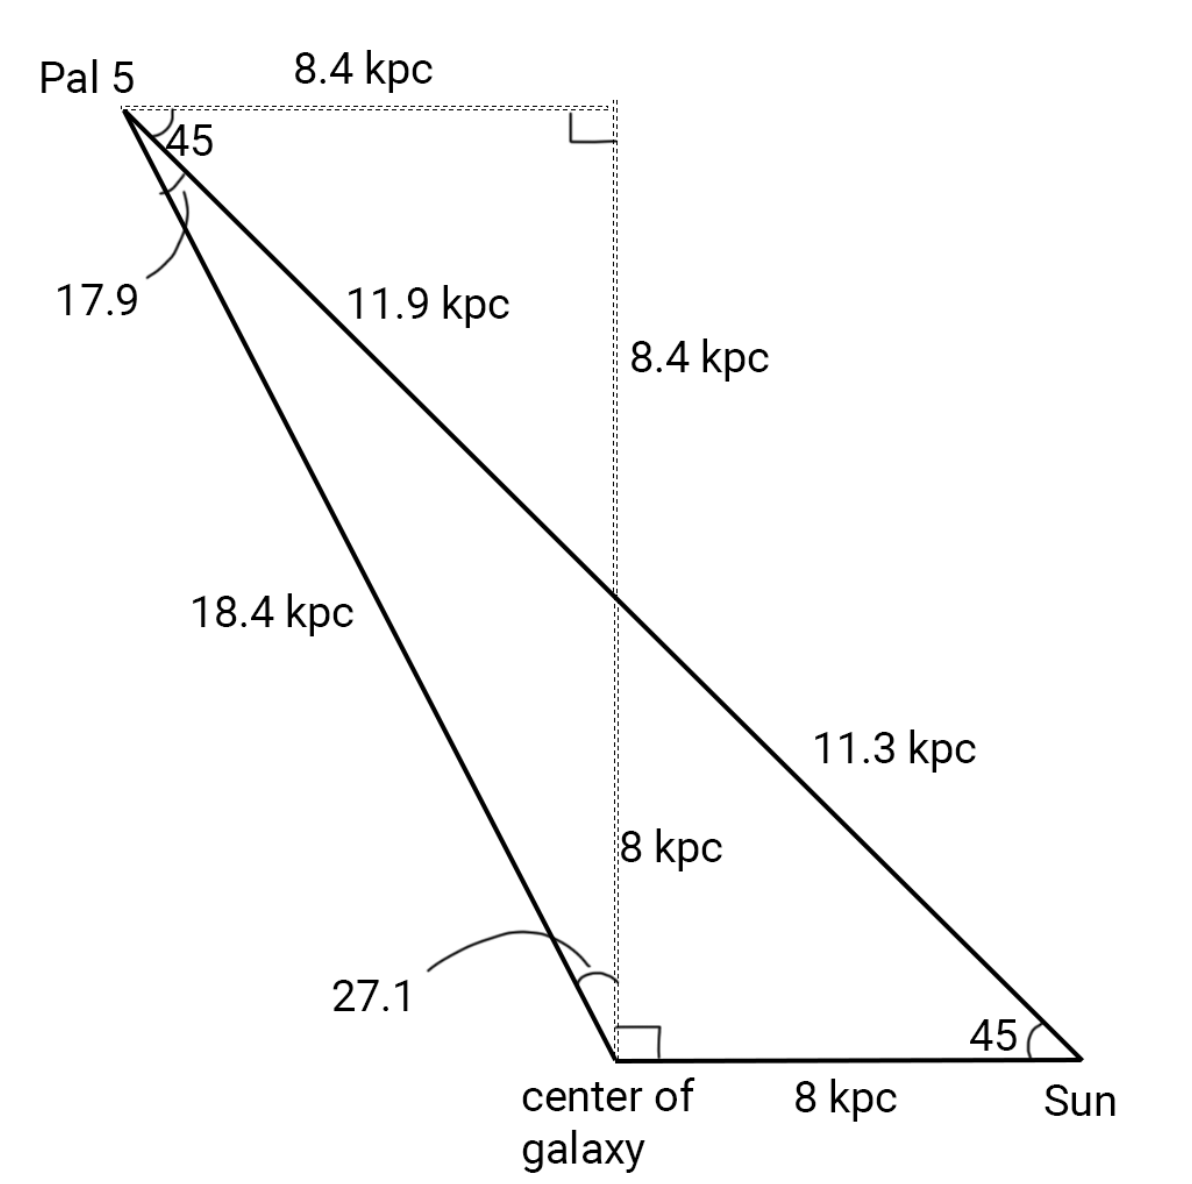
\includegraphics[width=0.4\linewidth]{trig.png}
        \caption{\label{fig:trig}Position of Pal 5 from a side-on view (the line connecting the center of the galaxy and the Sun is along the galactic disk). Units of angles are in degrees. Basic trigonometry was used to determine all the angles and lengths.}
    \end{figure}
    Knowing that the angle between the directional vectors from Pal 5 to the Sun and from Pal 5 to the center of the galaxy, and the fact that Pal 5, the center of the galaxy, and the Sun are all (very nearly) aligned, we can project the radial velocity vector (from Pal 5 to the Sun) in the direction of the vector from Pal 5 to the center of the galaxy. This gives the radial velocity from Pal 5 to the center of the galaxy:
        \begin{figure}[!htb]
            \centering
            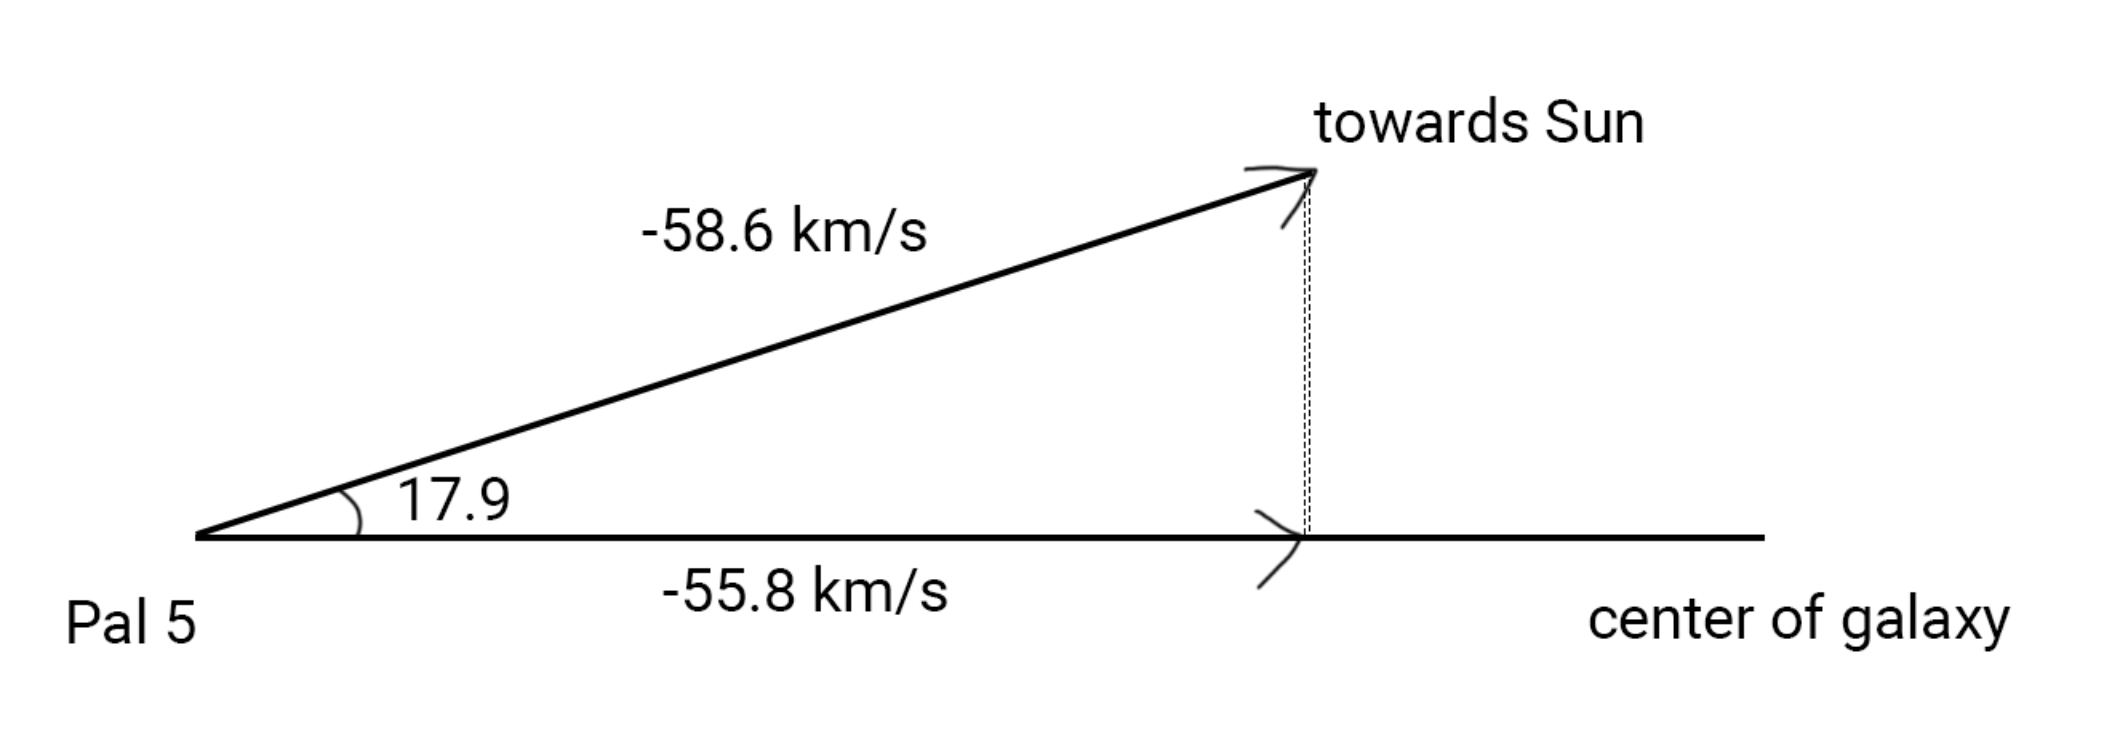
\includegraphics[width=0.5\linewidth]{projection.png}
            \caption{\label{fig:proj}Radial velocity of Pal 5 towards the center of the galaxy given by a projection of the vector representing radial velocity of Pal 5 towards the Sun: $v_{s2} = v_{s1} \cos(\theta) = -58.6~{\rm km\,s^{-1}}\cos{17.9^\circ} = -55.8~{\rm km\,s^{-1}}$.}
        \end{figure}
        Since the Sun is moving towards the center of the galaxy at $10~{\rm km\,s^{-1}}$, we need to make an adjustment of $10~{\rm km\,s^{-1}}\cos(45) = 7~{\rm km\,s^{-1}}$. So the radial velocity of Pal 5 towards the center of the galaxy is $-55.8~{\rm km\,s^{-1}} + 7~{\rm km\,s^{-1}} = -48.8~{\rm km\,s^{-1}}$.

        We can scale the tangential velocity observed from the Sun:
        \begin{align*}
            v_{t2} = v_{t1}\frac{d1}{d2} = 418.9~{\rm km\,s^{-1}}\frac{23.2~{\rm kpc}}{18.43~{\rm kpc}} = 528~{\rm km\,s^{-1}}.
        \end{align*}
        Then the total velocity is 
        \begin{align*}
            v = \sqrt{v_r^2 + v_t^2} = \sqrt{(-48.8~{\rm km\,s^{-1}})^2 + (528~{\rm km\,s^{-1}})^2} = 530~{\rm km\,s^{-1}}.
        \end{align*}

    \item Use Kepler's Third Law. Period given by 
        \begin{align*}
            P = \frac{2\pi R}{\Theta},
        \end{align*}
        where $R$ is distance from center, $\Theta$ is rotational velocity. Then assume mass of Pal 5 is negligible relative to the mass of the Milky Way. So 
        \begin{align*}
            M = \frac{4\pi^2R^3}{GP^2}.
        \end{align*}
    \end{enumerate}

\section*{Problem 7} 
\begin{enumerate}[label=(\alph*)]
    \item We start with the equations 
        \begin{align}
            v_r &= (\Omega - \Omega_0)R_0\sin(l) \\
            v_t &= (\Omega - \Omega_0)R_0\cos(l) - \Omega d.
        \end{align}
        For stars near the Sun, we perform a Taylor series approximation (first-order) of $\Omegea(R)$ about $\Omega_0(R_0)$:
        \begin{alignat}{2}
            &&\Omega(R) &\simeq \Omega_0(R_0) + \frac{d\Omega}{dR}\Big|_{R_0}(R-R_0) \nonumber \\
            \implies&&\Omega - \Omega_0 &\simeq \frac{d\Omega}{dR}\Big|_{R_0}(R-R_0).
        \end{alignat}
        Substituting Eq. 3 into Eq. 1, we obtain a new expression for $v_r$:
        \begin{align}
            v_r \simeq \frac{d\Omega}{dR}\Big|_{R_0}(R-R_0)R_0\sin(l).
        \end{align}
        We also know that 
        \begin{align}
            \Omega = \frac{\Theta}{R},
        \end{align}
        so the derivative $d\Omega/dR$ becomes
        \begin{align}
            \frac{d\Omega}{dR} = \frac{d(\frac{\Theta}{R})}{R} = \frac{\frac{d\Theta}{dR}R - \Theta}{R^2} = \frac{\frac{d\Theta}{dR}}{R} - \frac{\Theta}{R^2}.
        \end{align}
        Evaluating this at $R_0$ and multiplying by $R_0$ gives 
        \begin{align}
            R_0\frac{d\Omega}{dR}\Big|_{R_0} = R_0(\frac{\frac{d\Theta}{dR}\Big|_{R_0}}{R_0} - \frac{\Theta_0}{R_0^2}) = \left[\frac{d\Theta}{dR}\Big|_{R_0} - \frac{\Theta_0}{R_0}\right].
        \end{align}
        We can substitute this back in to Eq. 4:
        \begin{align}
            v_r \simeq \frac{d\Omega}{dR}\Big|_{R_0}(R-R_0)R_0\sin(l) = \left[\frac{d\Theta}{dR}\Big|_{R_0} - \frac{\Theta_0}{R_0}\right](R-R_0)\sin(l).
        \end{align}
        We can follow nearly identical steps for the tangential velocity. Performing (sequential) substitutions of Eq. 3 and Eq. 7 into Eq. 2, and using the approximation $\Omega \simeq \Omega_0$, we find that 
        \begin{align}
            v_t &= (\Omega - \Omega_0)R_0\cos(l) - \Omega d \\
            &= \frac{d\Omega}{dR}\Big|_{R_0}(R-R_0)R_0\cos(l) - \Omega d \\
            &= \left[\frac{d\Theta}{dR}\Big|_{R_0} - \frac{\Theta_0}{R_0}\right](R-R_0)\cos(l) - \Omega_0 d.
        \end{align}
    
    \item For the radial velocity, we start with Eq. 8:
        \begin{align}
            v_r = \left[\frac{d\Theta}{dR}\Big|_{R_0} - \frac{\Theta_0}{R_0}\right](R-R_0)\sin(l)
        \end{align}
        We multiply by $1/2$ and by $2$ (which doesn't change anything), and factor out $-1$ from the $(R-R_0)$ term:
        \begin{align}
            v_r = 2\times -\frac{1}{2}\left[\frac{d\Theta}{dR}\Big|_{R_0} - \frac{\Theta_0}{R_0}\right]\times(R_0-R)\sin(l).
        \end{align}
        Note that the second term is just $A$ (C&O Eq. 24.39):
        \begin{align}
            v_r = 2A(R_0-R)\sin(l).
        \end{align}
        Note also that for a small angle $\beta$, $\cos\beta \simeq 1$, so we have the approximation 
        \begin{align}
            d\cos(l) = R_0 - R\cos\beta \simeq R_0 - R.
        \end{align}
        Substituting this into Eq. 14, we have 
        \begin{align}
            v_r = 2A\sin(l)d\cos(l).
        \end{align}
        Reorganizing and using the identity $2\sin(l)\cos(l) = \sin(2l)$, we see that 
        \begin{align*}
            v_r = Ad\times 2\sin(l)\cos(l) = Ad\sin(2l)
        \end{align*}
        as expected.

        For the tangential velocity, we start with Eq. 11. As before, we multiply by $1/2$ and by $2$, and factor out $-1$ from the $R-R_0$ term:
        \begin{align}
            v_t &= 2\times -\frac{1}{2}\left[\frac{d\Theta}{dR}\Big|_{R_0} - \frac{\Theta_0}{R_0}\right]\times(R_0-R)\cos(l) - \Omega_0 d \\
            &= 2A\cos(l) - \Omega_0 d.
        \end{align}
        Making the same small angle approximation as before (Eq. 15), we get 
        \begin{align}
            v_t = 2A\cos(l)d\cos(l) - \Omega_0 d = Ad\times 2\cos^2(l) - \Omega_0 d.
        \end{align}
        Using the identity $\cos(2l) = 2\cos^2(l) - 1$, Eq. 19 becomes
        \begin{align}
            v_t &= Ad(\cos(2l) + 1) - \Omega_0 d \\
            &= Ad\cos(2l) + Ad - \Omega d \\
            &= Ad\cos(2l) + (A - \Omega)d.
        \end{align}
        Now, note the following:
        \begin{align}
            A - B &= -\frac{1}{2}\left[\cancel{\frac{d\Theta}{dR}\Big|_{R_0}} - \frac{\Theta_0}{R_0}\right] + \frac{1}{2}\left[\cancel{\frac{d\Theta}{dR}\Big|_{R_0}} + \frac{\Theta_0}{R_0}\right] \\
            &= \frac{1}{2}\frac{\Theta_0}{R_0} + \frac{1}{2}\frac{\Theta_0}{R_0} \\ 
            &= \frac{\Theta_0}{R_0} = \Omega_0.
        \end{align}
        In particular, we see that 
        \begin{alignat}{2}
            &&A - B &= \Omega_0 \\
            \implies&&A - \Omega_0 &= B.
        \end{alignat}
        Substituting this result into Eq. 22, we find that 
        \begin{align}
            v_t &= Ad\cos(2l) + (A - \Omega)d \\
            &= Ad\cos(2l) + Bd
        \end{align}
        as expected.

\end{enumerate}




\end{document}
